\section{Example Objects}

Totally tubular examples.  We are making

\subsection{Touch-sensitive Toy}

\begin{figure}[h]
\centering
    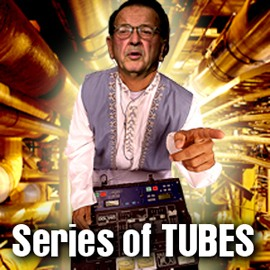
\includegraphics[width=3.4in]{figures/series-of-tubes.jpg}
\caption{A touch-sensitive rabbit whose tubes are filled with conductive paint.  Sensing is done on a single wire via SFCS.  Inset shows the internal structure of the tubes generated by our design tool.}
\label{fig:toy}
\end{figure}

We created a touch-sensitive toy and an app that goes along with it, reminiscent of the boat application in \cite{Harrison-acoustic}.  This toy has an interior star

\subsection{Braille Learning Tool}

\begin{figure}[h]
\centering
    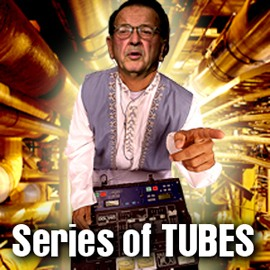
\includegraphics[width=3.4in]{figures/series-of-tubes.jpg}
\caption{This box has 6 individually-actuated semi-closed tubes capped with rubberlike material.  When air pressure is changed in these tubes, the caps inflate or deflate.  By actuating these tubes in particular sets, we can create braille letters.  Inset shows the internal structure of the tubes generated by our design tool.}
\label{fig:braille}
\end{figure}

\subsection{Custom Radio}

\begin{figure}[h]
\centering
    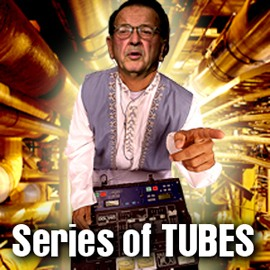
\includegraphics[width=3.4in]{figures/series-of-tubes.jpg}
\caption{This radio is assembled from traditional electronic components connected by copper-filled tubes.  The case was designed to allow the components to recess into it slightly.  Inset shows the internal structure of the tubes generated by our design tool.}
\label{fig:radio}
\end{figure}

\subsection{Presence-aware Pen Holder}

\begin{figure}[h]
\centering
    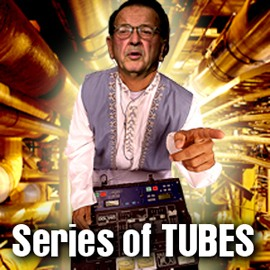
\includegraphics[width=3.4in]{figures/series-of-tubes.jpg}
\caption{This pen holder (a) uses Wimmer's FlyEye technique \valkyrie{can't add direct citation here??} (b) to sense the presence or absence of an object in each of its tubes.  Inset shows the internal structure of the tubes generated by our design tool.}
\label{fig:pens}
\end{figure}

\subsection{Animated Neon Sign}

\begin{figure}[h]
\centering
    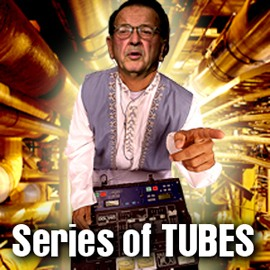
\includegraphics[width=3.4in]{figures/series-of-tubes.jpg}
\caption{A neon sign designed using our tool.  The tubes contains four separate electroluminescent wires, lit in sequence to create animation (a).  (b) shows the selections we made to generate our tube structures.  (c) shows the internal structure of the tubes generated by our design tool.}
\label{fig:neon}
\end{figure}